\section{Theory}
\subsection{Quality measures}
In simulation we are interested in producing meshes which consists of regular tetrahedrals or same sided triangles, which implies all sides and angles are equal. This means we are interested in creating uniform meshes which consists of correctly shaped tetrahedrals or triangles. We can use quality measures to assess our produced meshes and to compare which of two generated meshes are best. Simple quality measures could be the volume of our tetrahedrals, the surface area of our tetrahedrals / triangles or the inscribed sphere / circle of our tetrahedrals / triangles. These measure are quite simple but gives an indication to the uniformity of our mesh. However, these simple measures does not say anything about how we want the geometry to be, only if it is uniform. We thus use the paper \cite{Shewchuk} to find some better quality measures. As the title implies he lists quality measures for both interpolation and conditioning. We are not interested in the interpolation measures as we will not use our grids for numerical analysis, we will instead focus on conditioning measures. For our first experiment we will use two quality measure from \cite{Shewchuk}, namely what we will call 'volume over RMS of area' and 'radius ratio'. Both defined in table 7 and 8 on page 54-55. 'Volume over RMS of area' is defined as $\frac{3^{7/4}}{2\sqrt{2}}\frac{V}{A_{rms}^{3/2}}$ where $A_{rms}$ is the root mean square of the surface area of the tetrahedral. This gives a volume to surface area ratio. 'Radius ratio' is defined as $3\frac{r_{in}}{r_{circ}}$ where $r_{in}$ is the radius of the inscribed sphere radius and $r_{circ}$ is the circumscribed sphere radius. If this ratio is close to zero, it means the tetrahedral is very flat or very tall, and thus this measure can tell us about the angles in the tetrahedral. The last quality measure we will use has been found during study group work and will be called 'perfect regular tetrahedrals'. To get this measure we take a tetrahedral in our mesh and compute its volume. We then find the optimal side lengths for a tetrahedral of this volume, and we then compute the inscribed sphere radius of this optimal tetrahedral. We then compute the inscribed sphere radius of the original tetrahedral and compute the ratio between these two radii. This measure describes how close the side lengths in our tetrahedrals are to be optimal for their volume, i.e. how close the tetrahedrals are to be regular. All of these quality measures return values in the range 0 to 1 and can be considered fair as they return 0 for degenerate tetrahedrals.

\subsection{How to use wildmesh to generate meshes}
\textit{Wildmesh} is a python library which we can use to create meshes from .obj files. We first create a tetrahedralizer object which most notably takes as parameters \textit{stop\_quality} and \textit{max\_its} which impact the quality of the mesh which is gonna be generated. After creating the tetrahedralizer object we can load a .obj file and then compute the \textit{V} and \textit{T} matrices which encodes the coordinates of the vertices and the connectivity of the tetrahedrals. With these we can use the library \textit{meshplot} to show the meshes. The result 'tetrahedralizing' the 'dragon.obj' and 'knot.obj' files can be seen in \autoref{wildmesh} and the Armadillo can be seen in experiment 1.
\begin{figure}[H]
	\centering
	\begin{subfigure}[b]{0.49\linewidth}
		\centering
		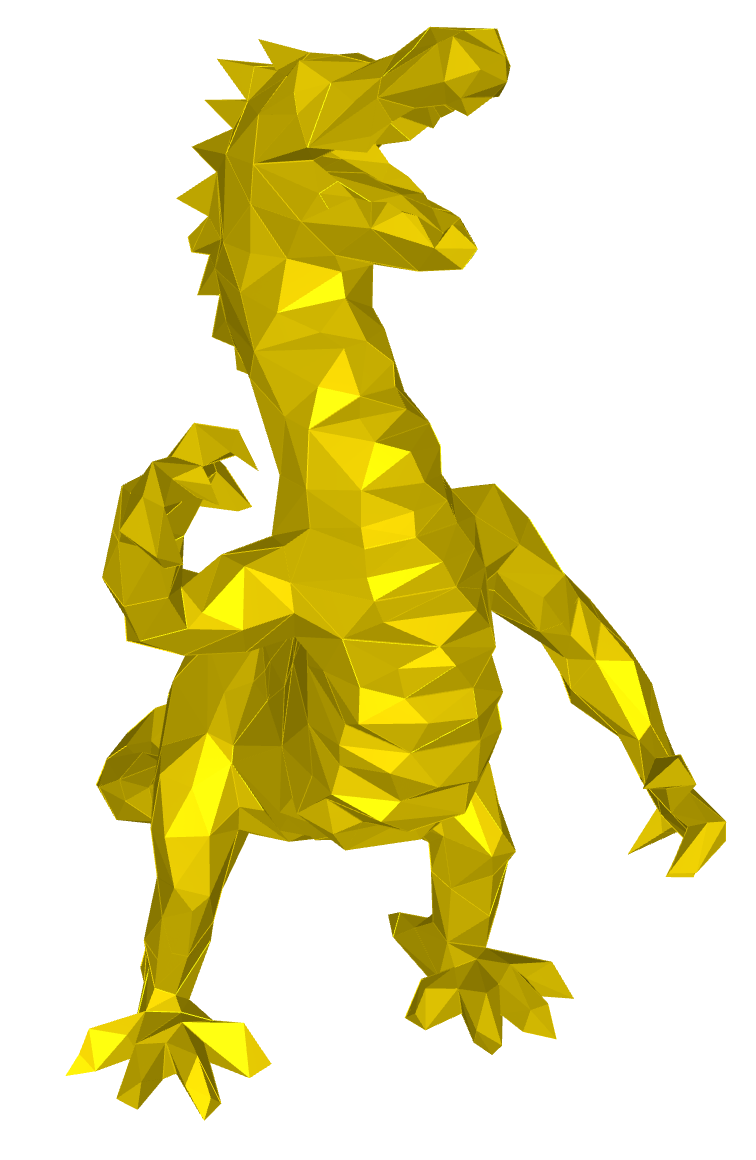
\includegraphics[height=0.75\linewidth]{Materials/dragon}
		\caption{Wildmesh generated mesh for 'dragon.obj'.}
	\end{subfigure}
	\hfill
	\begin{subfigure}[b]{0.49\linewidth}
		\centering
		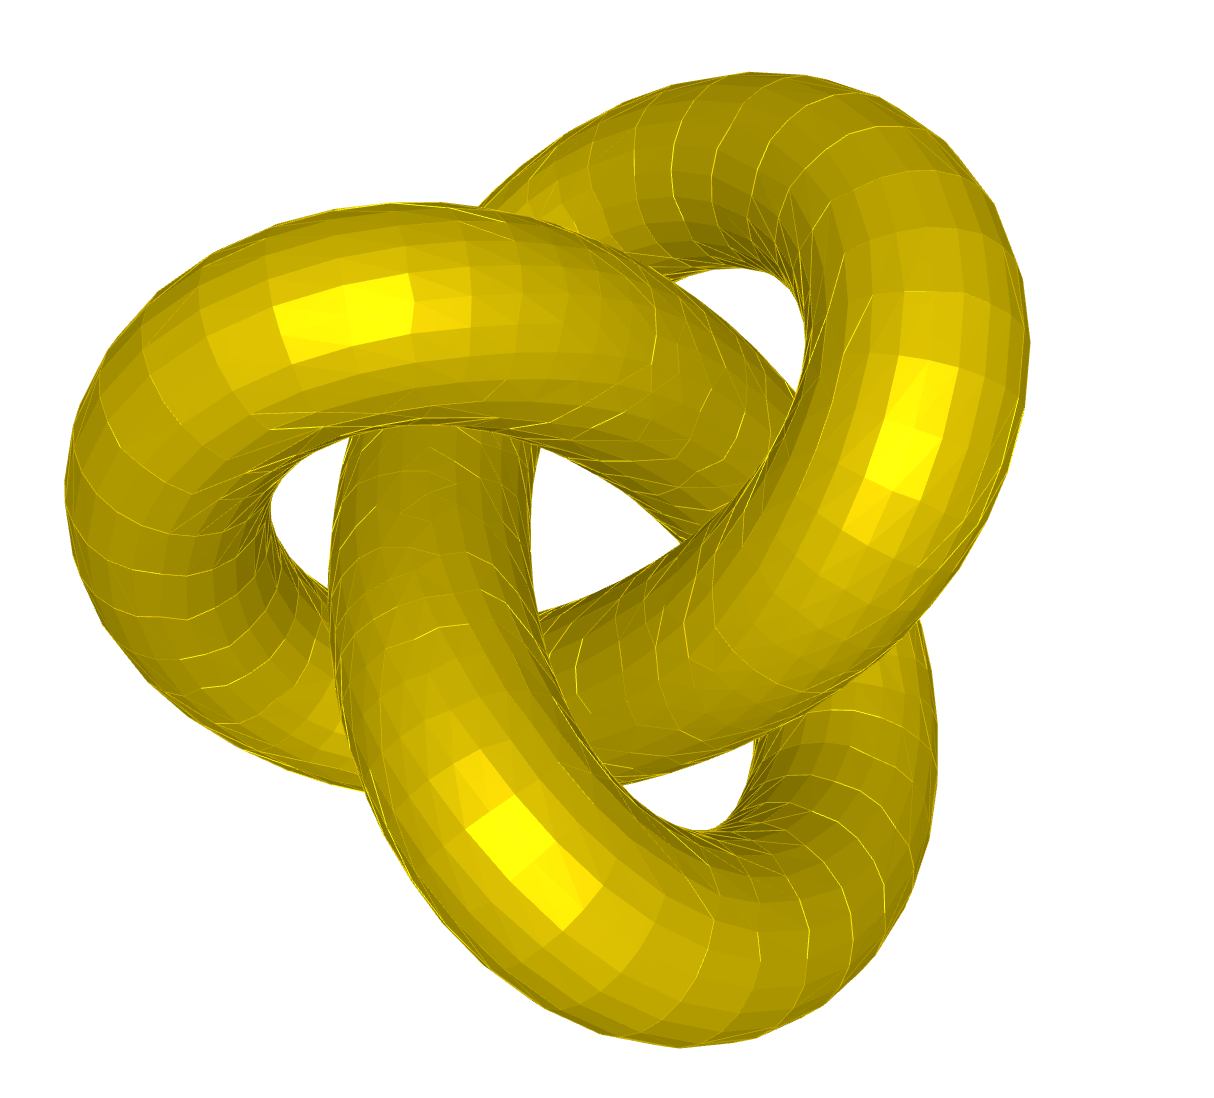
\includegraphics[height=0.75\linewidth]{Materials/knot}
		\caption{Wildmesh generated mesh for 'knot.obj'.}
	\end{subfigure}
	\caption{Wildmesh generated meshes.}
	\label{wildmesh}
\end{figure} 